\documentclass{beamer}

\usetheme{Warsaw}
\definecolor{indigo(web)}{rgb}{0.29, 0.0, 0.51}
\usecolortheme[named=indigo(web)]{structure}

% used for lines in tables
\usepackage{booktabs}


% package for including source code
% https://en.wikibooks.org/wiki/LaTeX/Source_Code_Listings
% http://mirrors.fe.up.pt/pub/CTAN/macros/latex/contrib/listings/listings.pdf
\usepackage{listings}


\title[Improving reproducibility in building simulation]{Improving reproducibility in building simulation: a pure-Python approach to geometry creation}
\author{Steven Firth}
\institute{Loughborough University}
\date{2021-06-23}

\begin{document}
	
	\begin{frame}
		\maketitle
	\end{frame}
	
	\begin{frame}{My background}
		\begin{itemize}
			\item I joined Loughborough University in 2008
			\item My job title is Reader in Building Performance Modelling
			\item I teach building simulation, energy data analysis, sustainable building design and renewable energy.
			\item I was a member of the University's Open Research Working Group in 2019.
			\item I was awarded the CALIBRE Winter 2019 Award for Open Research
			\item In 2015 I published the Refit Smart Home dataset on the University's Data Repository (14,307 views, 3,997 downloads)
			\item I publish papers on FAIR data and open research methods using Python and Jupyter Notebooks 
			\item I maintain the GitHub pages for the Building Energy Research Group
			
		\end{itemize}
	\end{frame}
	
	\begin{frame}{The problem I am trying to solve}
		\begin{itemize}
			\item \textbf{Task:} I would like \emph{to construct a building simulation model} of a 4 bed house and \emph{to simulate the energy performance} of the house using the EnergyPlus software.
			\item \textbf{Challenge:} I would like to do this in an \emph{open, transparent} way so that the whole process is \emph{reproducible}. 
		\end{itemize}
	\end{frame}

	\begin{frame}{What is "Reproducible"?}
		The Alan Turing Institute in its publication 'The Turing Way' defines reproducible research for data science as: \\ [10pt]
		\begin{quote}
			Work that can be independently recreated from the same data and the same code that the original team used. 
		\end{quote}
	\end{frame}

	\begin{frame}{An Example of Reproducibility}
		This presentation is reproducible as it is written in code (Latex)\\[10pt]
		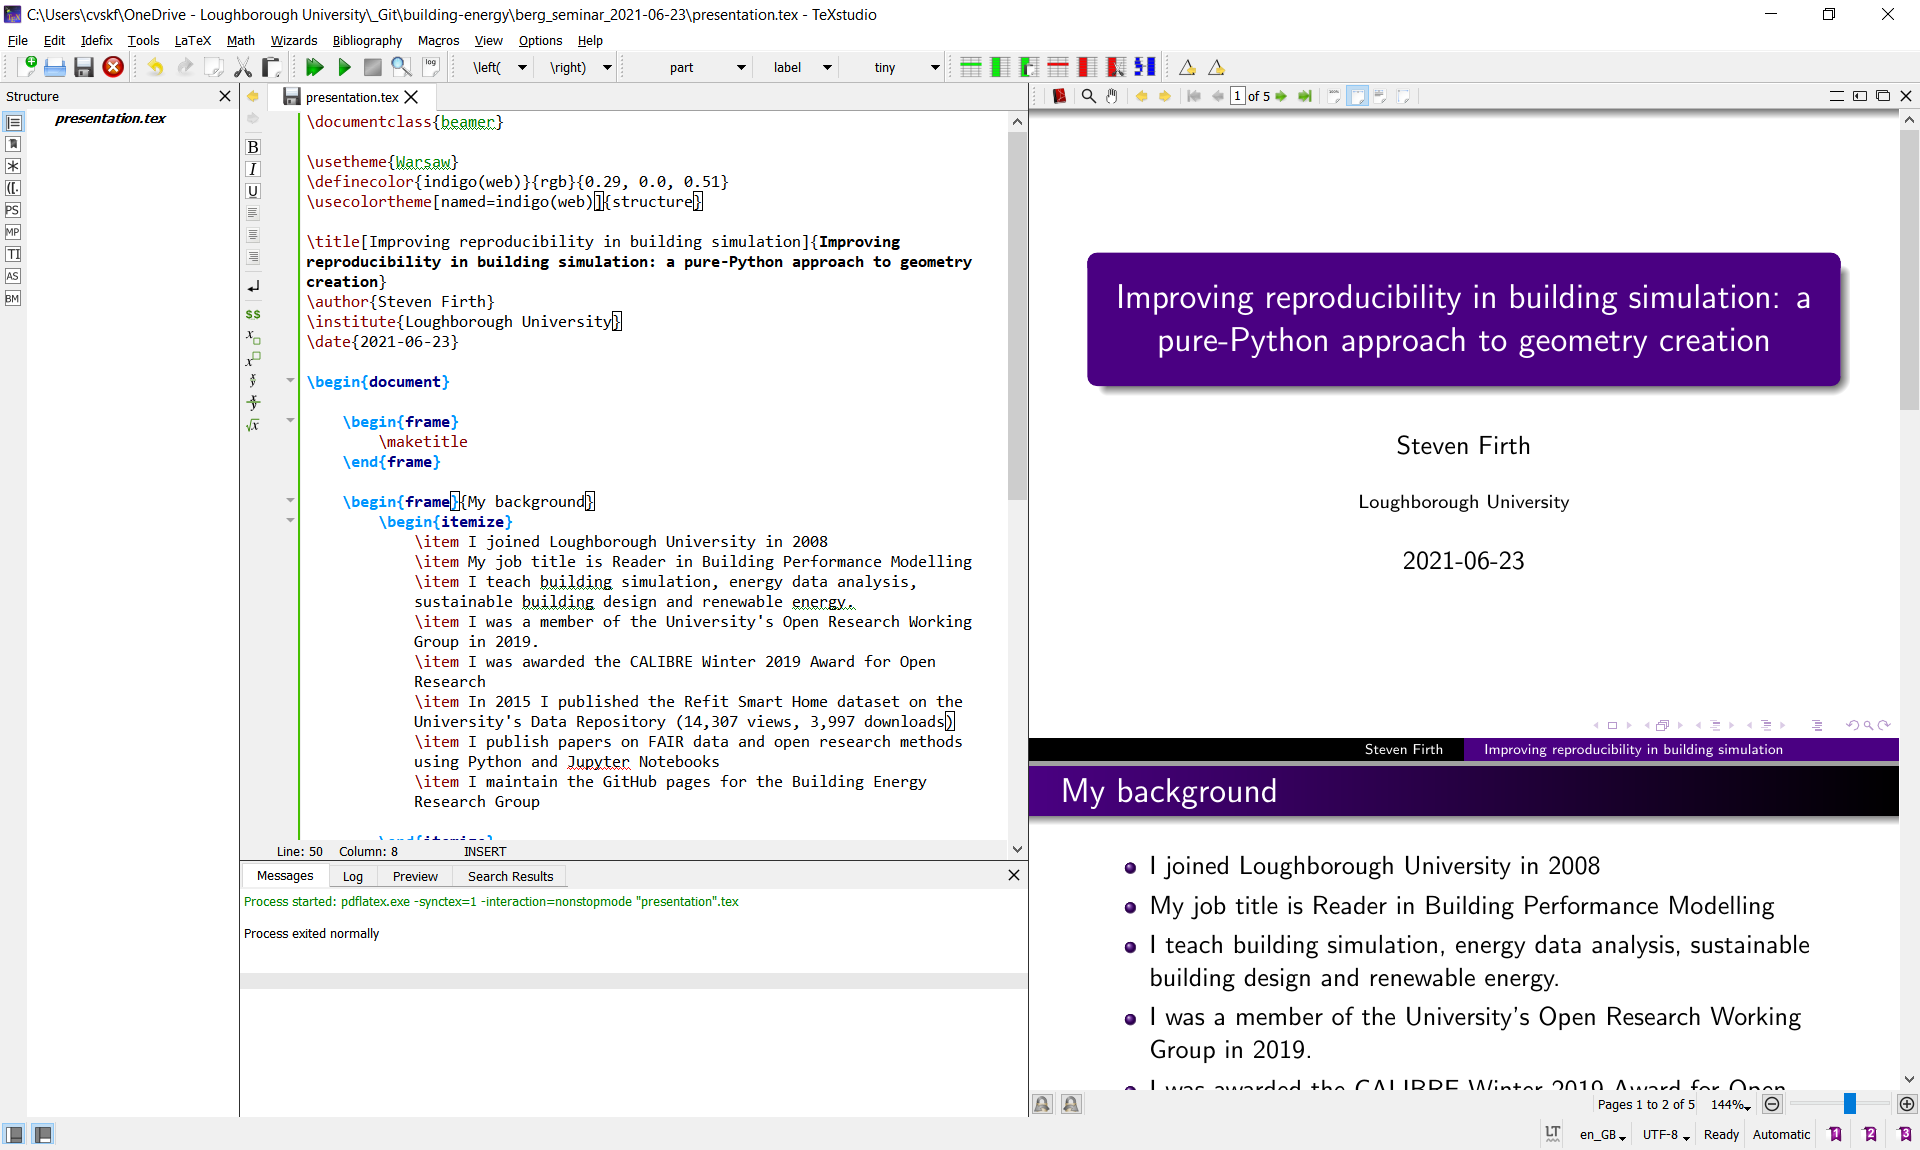
\includegraphics[width=\textwidth,keepaspectratio]{latex_example.png}
	\end{frame}
	
	\begin{frame}{An Example of Open Reproducibility}
		This presentation is also open as the code is hosted on the BERG Github repository\\[10pt]
		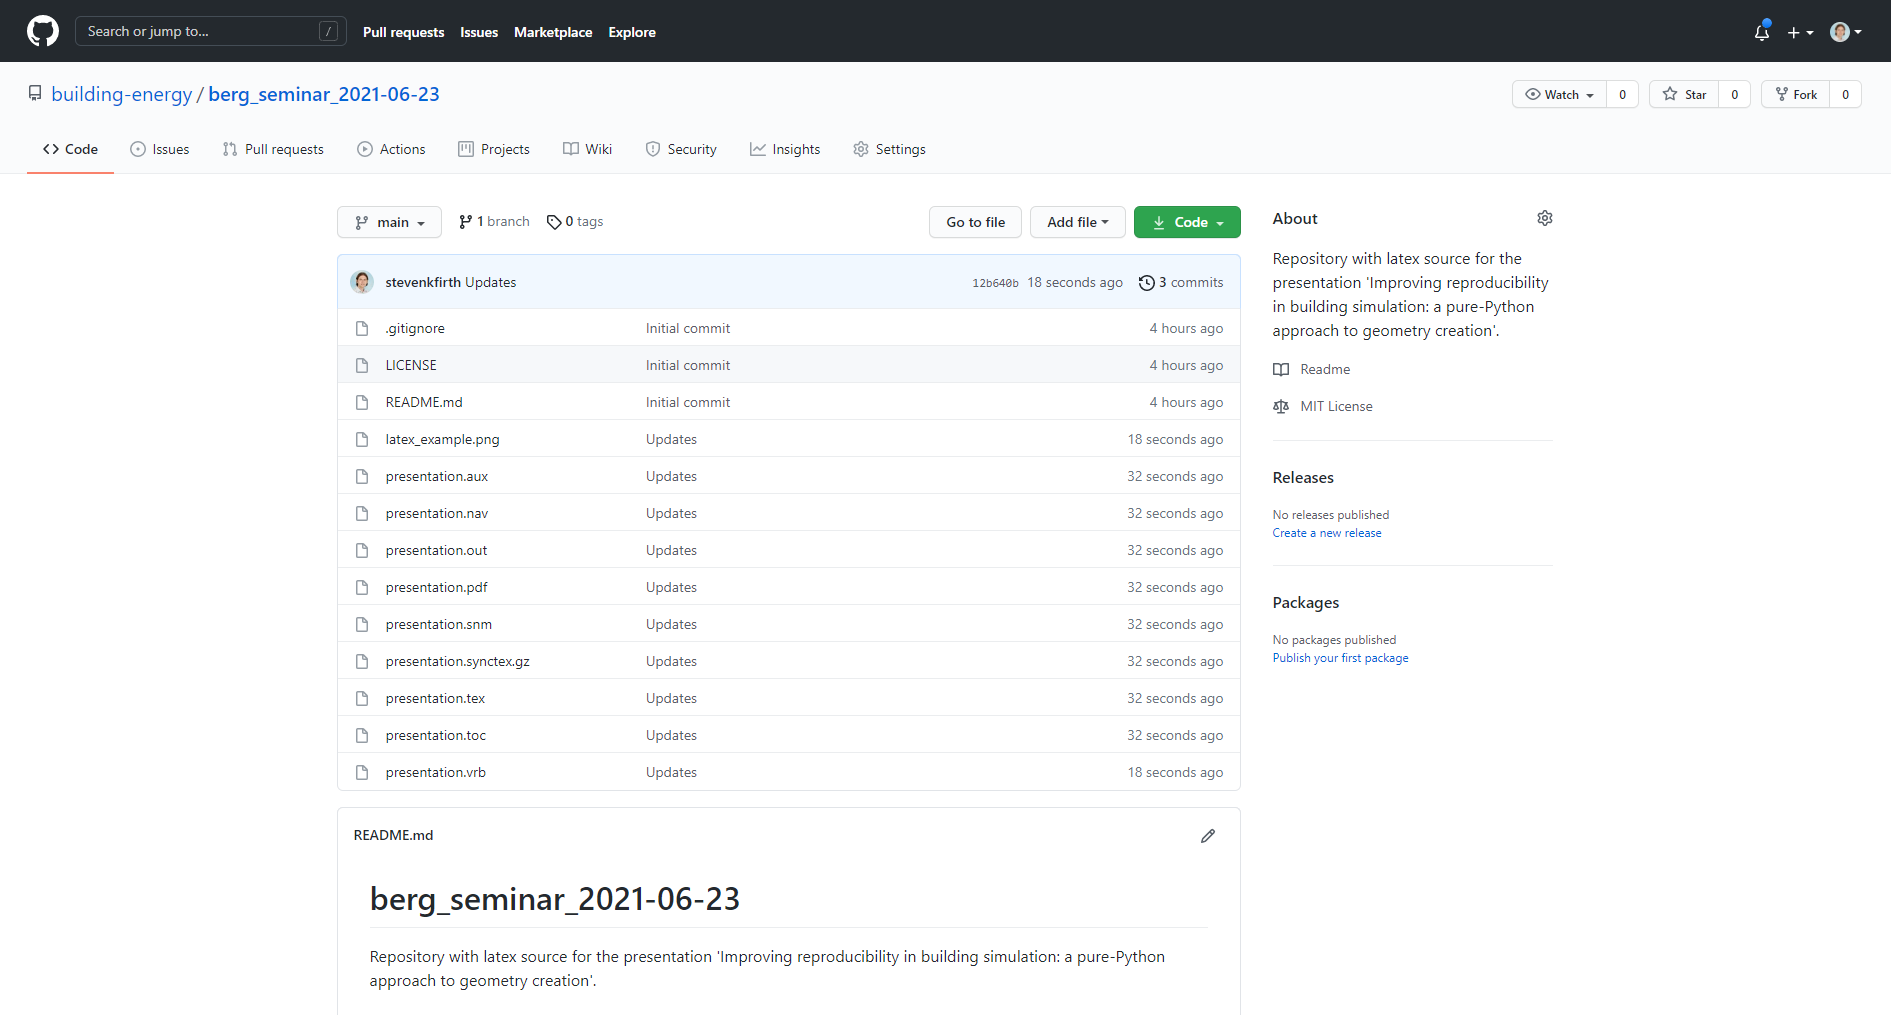
\includegraphics[width=\textwidth,keepaspectratio]{github_example.png}
	\end{frame}

	\begin{frame}{Point-and-click vs. Text-based commands}
		\hyphenpenalty=100000
		\begin{tabular}{p{0.3\textwidth}p{0.3\textwidth}p{0.3\textwidth}}
			 \toprule
			 Research task & Point-and-Click & Text-based Commands \\
			 \midrule
			 Writing documents & Microsoft Word, Apple Pages & \LaTeX \\
			 Creating slides & Microsoft PowerPoint, Apple Keynote & \LaTeX \\
			 Analysing data & Microsoft Excel, Google Sheets & Python and Jupyter Notebooks \\
			 Building websites & Adobe Dreamweaver & HTML, Bootstrap, Django
		\end{tabular}
	\end{frame}

	\begin{frame}{Geometry Creation - Case Study}
		\includegraphics[width=\textwidth,keepaspectratio]{"C:/Users/cvskf/OneDrive - Loughborough University/_Git/stevenkfirth/PythonGeometryPaper/4_1_Case_Study_Single_Zone_with_Window/Fig_4_1a".jpeg}
	\end{frame}

	\begin{frame}{Creating geometry using Python}
		\footnotesize
		\lstinputlisting[language=Python, numbers=left, xleftmargin=2em, frame=single, framexleftmargin=2em]{"C:/Users/cvskf/OneDrive - Loughborough University/_Git/stevenkfirth/PythonGeometryPaper/4_1_Case_Study_Single_Zone_with_Window/4_1_code.py"}
	\end{frame}

	\begin{frame}{Conclusions}
		\begin{enumerate}
			\item Reproducibility involves writing text-based commands, i.e. code, scripts, programming etc.
			\item The challenge in developing building simulation models using text-based commands is the 3D geometry of the building model.
			\item New open source libraries and packages are required for tasks such as:
			\begin{itemize}
				\item Doing geometry calculations (i.e. 3D polygon intersection, 3D polyhedron intersection)
				\item Working with BIM models that contain geometric and non-geometric data (construction, internal gains etc.)
				\item Interfacing with standard building simulation file formats (gbXML, idf, epJSON)
			\end{itemize} 
		\end{enumerate}
	\end{frame}

	
\end{document}